%% Dokumentklasse KOMA-Script Report
\documentclass[paper=a4, 12pt]{scrreprt}
%% Encoding UTF8
\usepackage[utf8]{inputenc}
%% 8 Bit Aufloesung der Buchstaben
\usepackage[T1]{fontenc}
%% Seitenraender
\usepackage[scale=0.85]{geometry}
%% Spracheinstellungen
\usepackage[english, naustrian]{babel} % your native language must be the last one!!
%% erweiterte Farbenpalette
\usepackage[dvipsnames]{xcolor}
%% Abbildungen
\usepackage{float}
\usepackage{adjustbox}
%% Tabellen (erweitert)
\usepackage{tabularx}
%% TikZ + Circuit-TikZ (fuer Schaltungen)
\usepackage[europeanresistors, europeaninductors]{circuitikz}
%% Nuetzliche TikZ Libraries
\usetikzlibrary{arrows, automata, positioning}
%% mathematik
\usepackage{amsmath, amssymb}
%\usepackage{mathtools}	
%% pdf-einbindung
\usepackage{pdfpages}
%% scource-code einbindung
\usepackage{listings, scrhack} %scrhack vermeidet Umschaltung auf KOMA Floats..
\usepackage{courier}
%% euro-symbol
\usepackage{eurosym}
%% landcsape-seiten ermöglichen
\usepackage{lscape}

%% Diplomarbeits-Format
\usepackage{srdpdipa}

%% Abkuerzungsverzeichnis
\usepackage[]{acronym}

%% Todos
\usepackage[]{todonotes}

%% Ganttdiagramme
\usepackage{pgfgantt}

%% Subfigures
\usepackage[lofdepth]{subfig}

%% definitionen =====================================%%
\dataSchool{HTBLuVA St. Pölten}
\dataDepartment{Höhere Lehranstalt für Elektronik und Technische Informatik}
\dataSubdepartment{Ausbildungsschwerpunkte Embedded Systems}
\dataSession{2019/20}

\title{CAN-Bus gesteuerte Stromquelle}
\author{Florian Hintermeier \and Dominik Gansch}
\date{\today}
\place{St. P\"olten}
\professor{Dipl.-Ing. Josef Radlbauer}
%%====================================================%%

% Hyperlinks im Dokument
\usepackage[colorlinks=true,
    linkcolor=black,
    citecolor=green,
    bookmarks=true,
    urlcolor=black,
    bookmarksopen=true]{hyperref}

\begin{document}

\frontmatter

%% titelseite ==========================================%%
\maketitle
%%======================================================%%

%% komplett leere seite ================================%%
%%\newpage\null\thispagestyle{empty}\newpage
%%======================================================%%

%% eidesstattliche erklärung ===========================%%
%%\begin{affidavit}
%%    \unterschrift{Florian Hintermeier}
%%    \unterschrift{Dominik Gansch}
%%\end{affidavit}
%%======================================================%%

%% dokumentation (deutsch/englisch) ====================%%
%%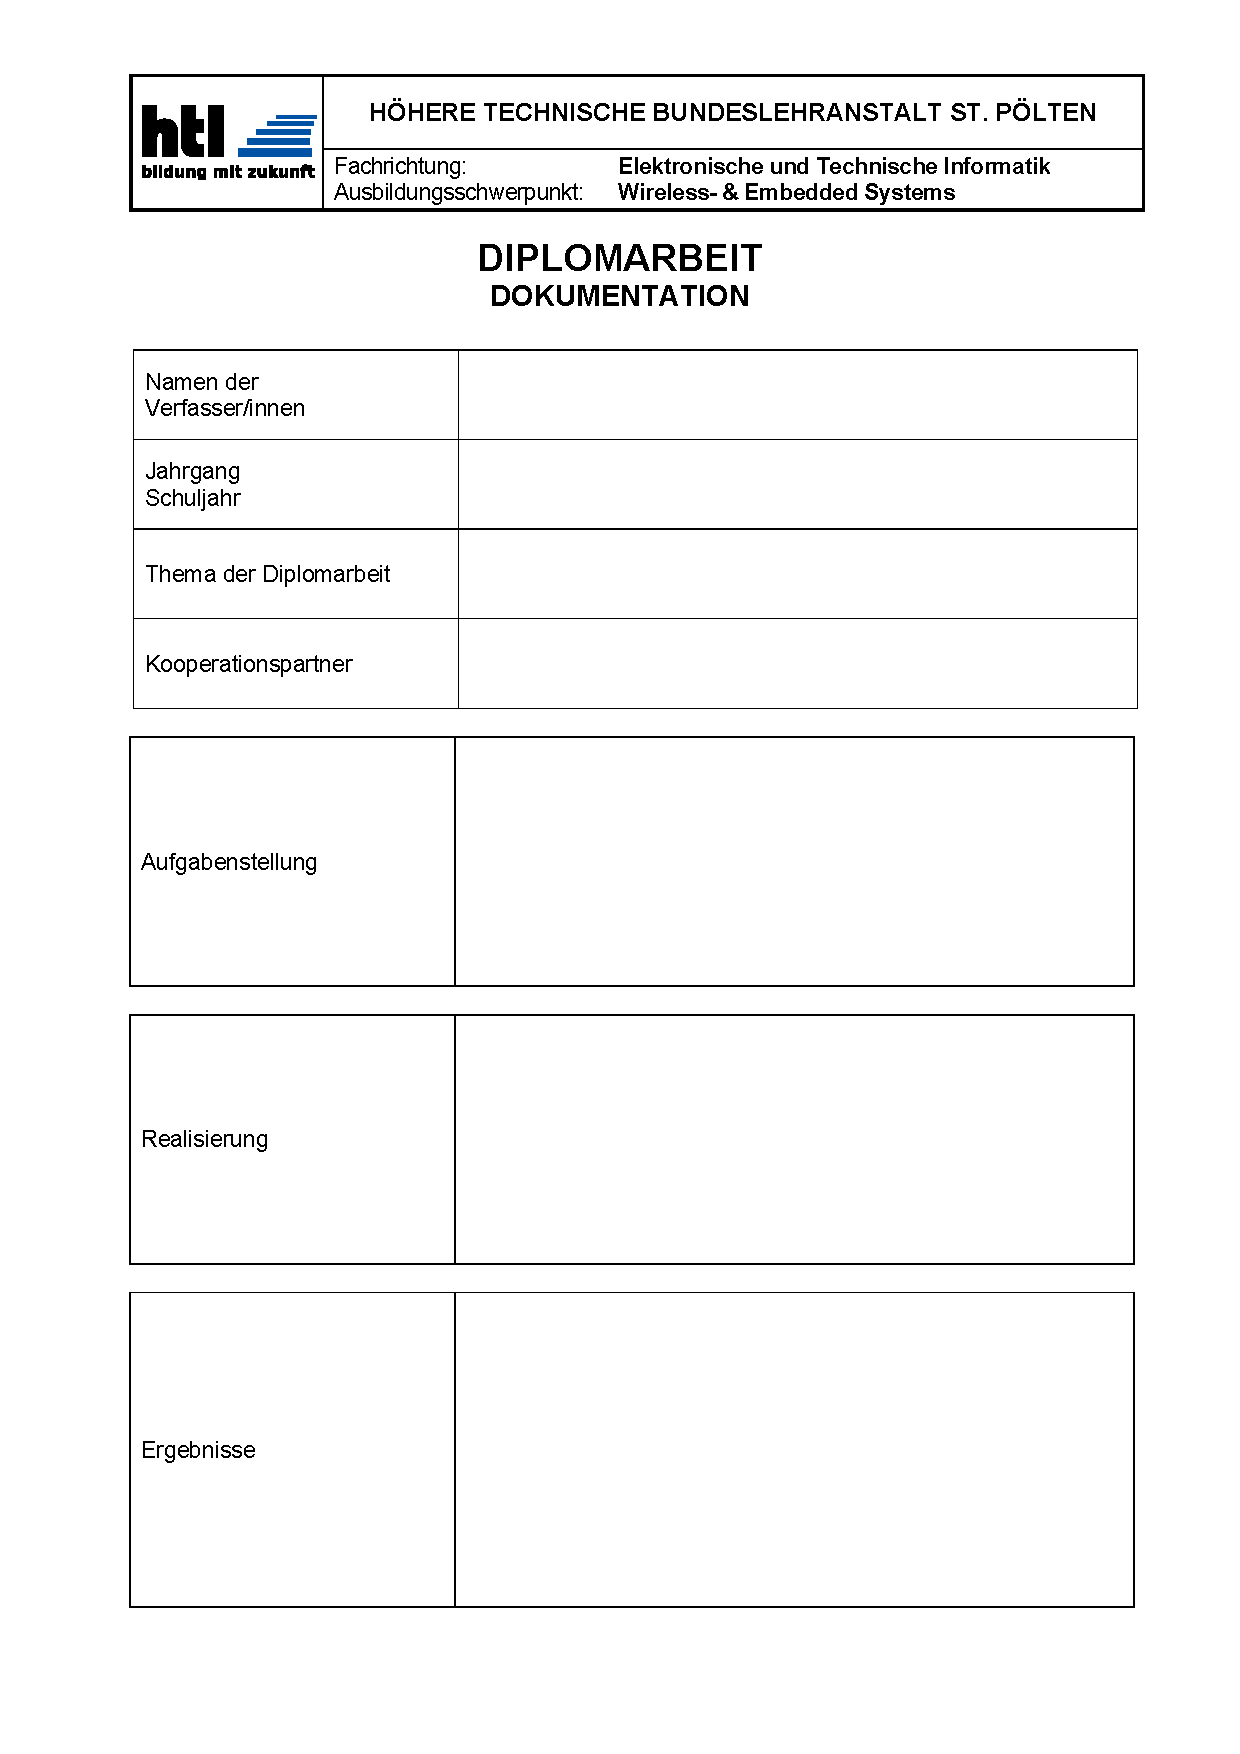
\includepdf[pages=-]{form/dokumentation-de.pdf}
%%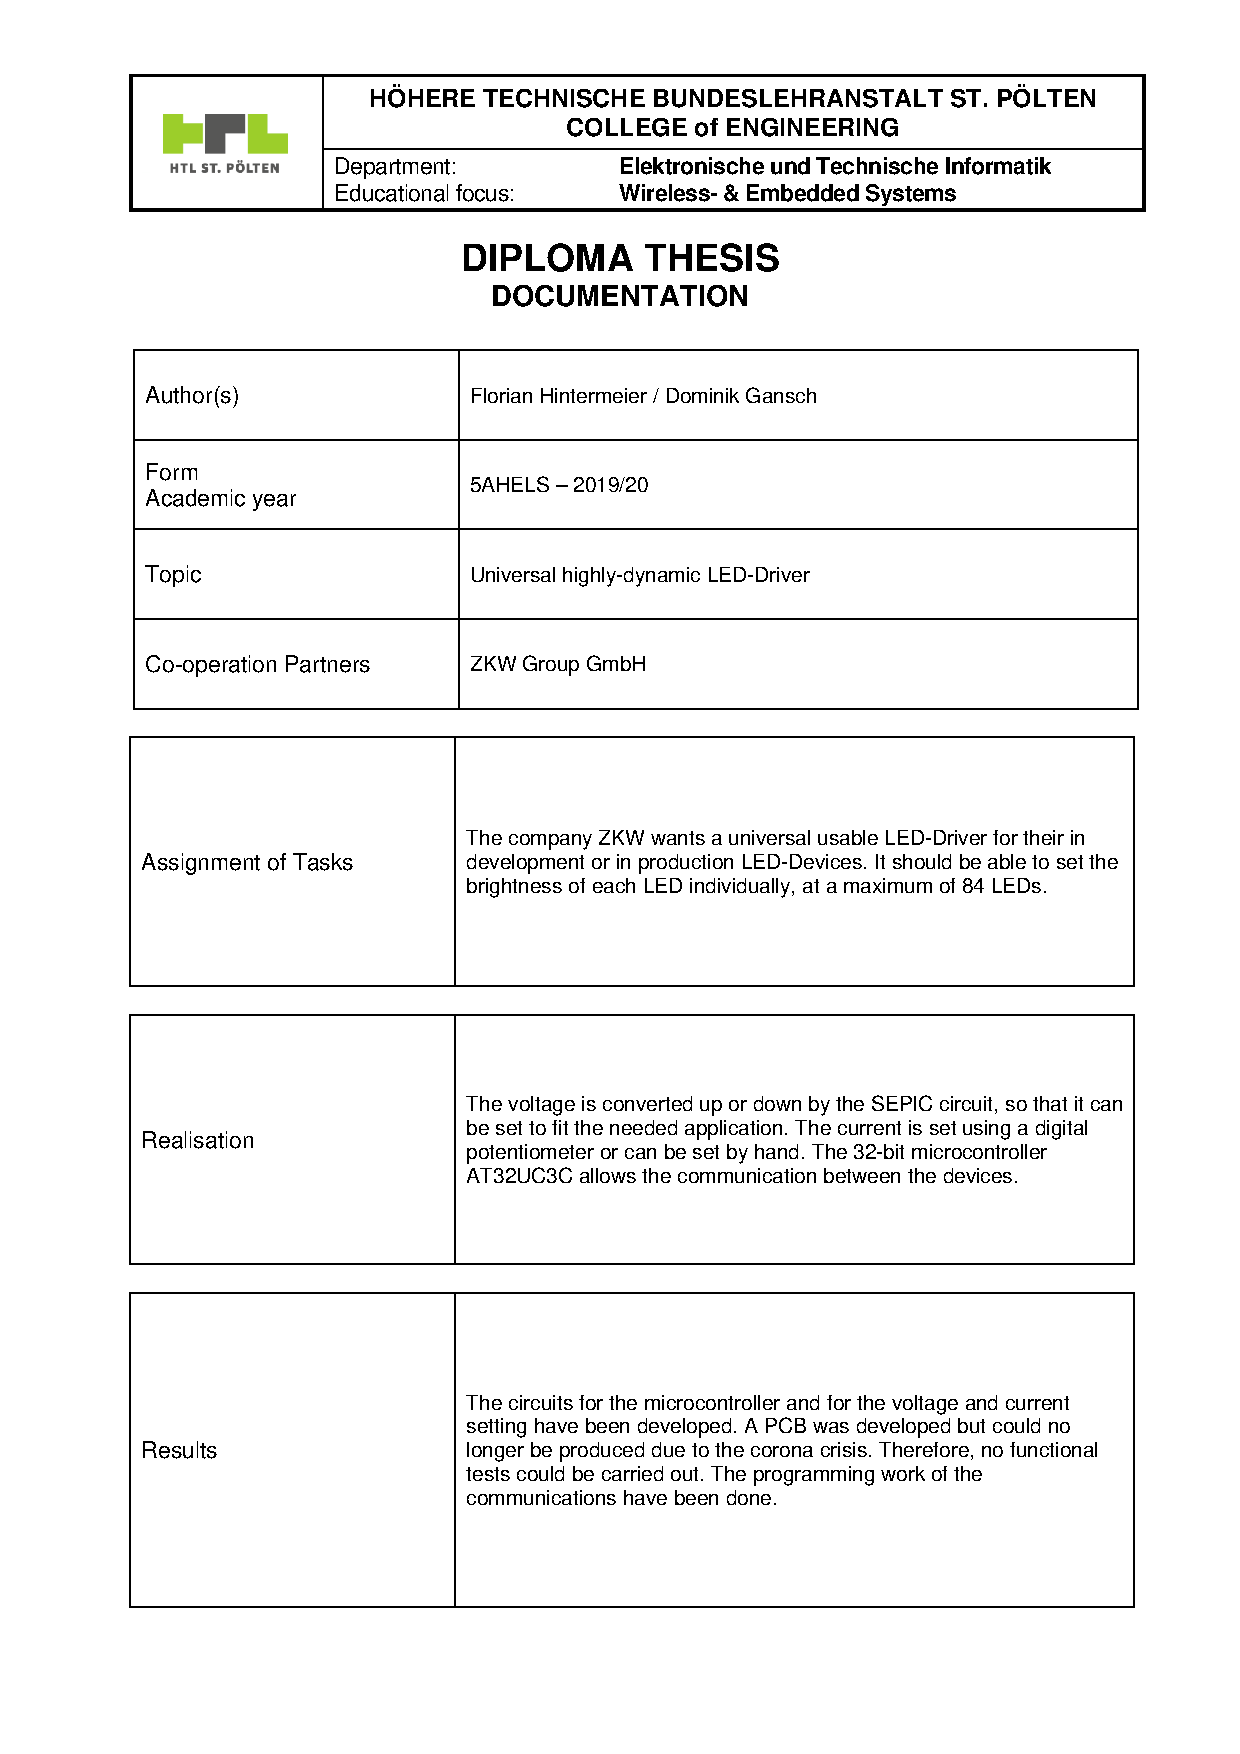
\includepdf[pages=-]{form/dokumentation-en.pdf}
%%======================================================%%

%% inhaltsverzeichnis ==================================%%
\tableofcontents
%%======================================================%%

%% HAUPTTEIL ===========================================%%
\responsible{Florian Hintermeier, Dominik Gansch}
\mainmatter

\chapter{Einleitung}
    Die Firma ZKW möchte für zahlreiche in Entwicklung und bereits in Produktion befindliche LED Einheiten einen universell einsetzbaren LED Treiber mit linear einstellbarem Strom. Dabei soll jede einzelne LED von maximal 84 individuell in ihrer Helligkeit eingestellt werden können.
    
	\begin{adjustbox}{center,caption={Blockschaltbild von ZKW},label={ZKW-Blockschaltbild},nofloat=figure,vspace=\bigskipamount}
	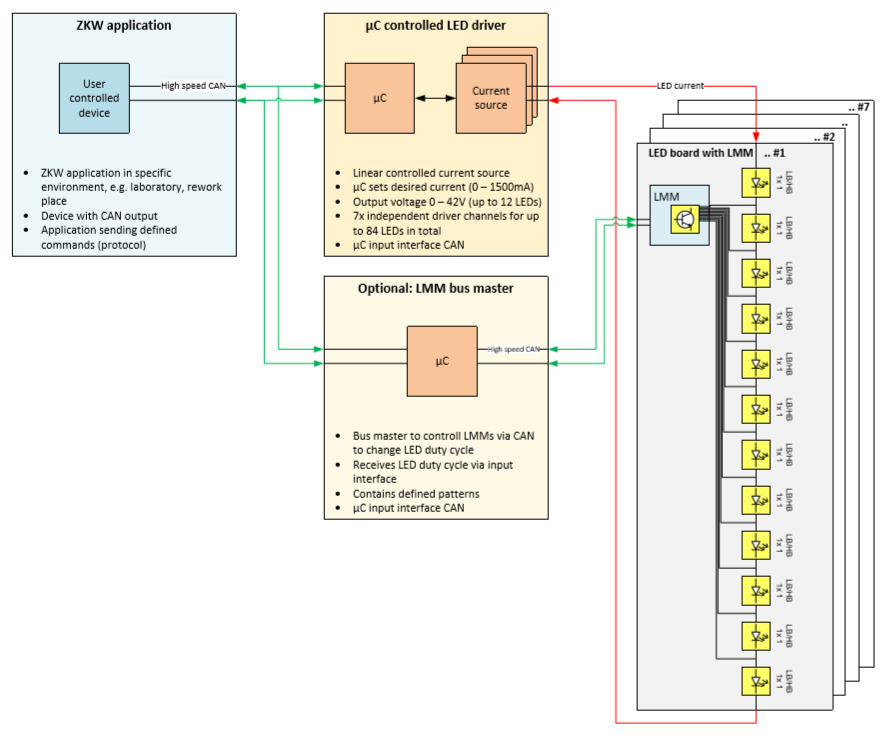
\includegraphics[width=\textwidth]{img/ZKW_Blockschaltbild.PNG}
	\end{adjustbox}

	Das Ziel liegt darin, eine geeignete Schaltung zu entwickeln um den von ZKW gegebenen Anforderungen zu entsprechen. Zu sehen sind diese in Abbildung 1.1.

\chapter{Individuelle Zielsetzung}
    \section{Hardware}    	
    	\subsubsection{Analogteil}
        Dieser Teil wird von Florian Hintermeier entwickelt. Er enthält die Schaltung um die Angeforderten Spannungen und Ströme erzeugen zu können, die von einem Mikrocontroller eingestellt werden sollen.
        
        \subsubsection{Digitalteil}
        Dieser Teil wird von Dominik Gansch entwickelt. Der Digitalteil dient als zentrale Steuerungseinheit. Das Kernstück des Digitalteils besteht aus dem Mikrocontroller, welcher über CAN-Bus Befehle (von der ZKW-Application) bestimmte Kommandos erhält. Die CAN-Befehle kann man in zwei Gruppen einteilen, in Befehle für die LMMs und in Stromregelungsbefehle. Für jedes LMM-Kommando gibt es im Mikrocontroller eine entsprechende Lichtbild-Ablauf-Tabelle, diese Daten der Tabelle werden, nach erhalten des dafür entsprechenden Befehls, laufend zu den LMMs gesendet und von diesen umgesetzt, bis der Lichbild-Ablauf abgeschlossen ist. Befehle für die Stromregelung werden mithilfe des internen DACs in einen Spannungsreferenzwert für die Stromregelung umgesetzt.    
    %%\section{Software}

\chapter{Grundlagen und Methoden}
	\section{Verwendete Software}
	Die hier aufgeführte und kurz erklärte Software wurde für die Erreichung der Ziele in diesem Projekt verwendet.
	
	\paragraph{LTSpice}\hfill \break
	LTspice ist eine kostenlose Software des ehemaligen Halbleiterherstellers Linear Technology (seit 2017: Analog Devices) zur Schaltungssimulation. Es basiert auf SPICE, ist dazu kompatibel und besonders zur Simulation von Schaltnetzteilen geeignet. Entwickelt und gepflegt wird es von Mike Engelhardt.\footnote{https://de.wikipedia.org/wiki/LTspice}
	\paragraph{Draw.io}\hfill \break
	Draw.io stellt sich als ein technisch anspruchsvolles Diagramm-Tool vor, das im Browser arbeitet und Modellierungssprachen wie UML, ERM und BTPM unterstützt. Die Standard-Version ist kostenlos.\footnote{https://www.tecchannel.de/a/draw-io-kostenloses-diagramm-tool-fuer-den-browser,2078028}
	\paragraph{Altium Designer 19}\hfill \break
	Eines der Hauptziele von Altium ist es, eine integrierte Entwicklungslösung zur Elektronikentwicklung anzubieten.
	Altium Designer beinhaltet die Schaltbildeingabe, einen PCB Layout Editor mit Integritätsanalyse sowie eine auf SPICE-Modellen gestützte Schaltungssimulation.\footnote{https://de.wikipedia.org/wiki/Altium\_Designer}\\
	In diesem Projekt wurde es dazu verwendet, um die Schaltungen zu Zeichnen und das PCB damit zu erstellen.
	\paragraph{TeXstudio}\hfill \break
	TeXstudio ist ein LaTeX-Editor für Windows, Linux, BSD und (Mac) OS X. Er ist open source und basiert auf Texmaker. Wie andere bekannten LaTeX-Editoren bietet auch er die grundlegende Unterstützung beim Einfügen von LaTeX-Befehlen, Syntax-Hervorhebung, eine integrierte Vorschaufunktion und eine Projektfunktion.\footnote{https://latex.tugraz.at/programme/texstudio}
	\newpage
	
	\section{Basis des Analogteils}
	Die Basis des Analogteils bildet eine SEPIC Schaltung, das Funktionsprinzip wird unten Beschrieben.
	\paragraph{SEPIC Funktionsprinzip}\footnote{https://www.elektroniknet.de/elektronik-automotive/sonstiges/sepic-wandler-fuer-automotive-anwendungen-1571.html}\hfill \break
	Die Anstiegssteilheit der Ströme IL1 und IL2 hängen von der Eingangsspannung und von den Induktivitätswerten der Spulen ab. Wenn der Schalter (Q) geschlossen wird, liegt an L1 die Eingangsspannung und an Cs eine Spannung, die genau so groß wie die Eingangsspannung ist. Der Strom steigt in den Spulen L1 und L2 an und Energie wird in den Spulen gespeichert. In dieser Zeit wird die Diode D in Sperrrichtung betrieben und der Ausgangskondensator muss den Strom für die angeschlossene Last liefern. Wenn der Schalter geöffnet wird, kehrt sich die Polarität der Spannung an den Spulen um. Die Diode leitet nun die gespeicherte Energie an den Ausgangskondensator und an die angeschlossene Last.
	\begin{adjustbox}{center,caption={Prinzipschaltung eines SEPIC-Converters},label={fig:SEPIC-Prinzipschaltung},nofloat=figure,vspace=\bigskipamount}
		\includegraphics[height=10cm]{img/SEPIC_PRinzipschaltung.jpg}
	\end{adjustbox}
	
\chapter{Ergebnisse}
	\section{Analogteil}
	Da die Eingangsspannung mit der das Gerät versorgt werden soll, zwischen 10 und 15 Volt liegt, muss man die Spannung erhöhen, was in diesem Fall mit einem SEPIC-Converter passiert. Als Basis dafür wurde der LT3757 Verwendet.\hfill \break
	Die Grundbeschaltung wurde aus dem Datenblatt\footnote{https://www.analog.com/media/en/technical-documentation/data-sheets/3757Afe.pdf Seite 31} übernommen, die benötigten Bauteilwerte wurden jedoch mittels Simulationen mit LTSpice ermittelt. 
	\begin{adjustbox}{center,caption={Referenzschaltung für SEPIC}, label={fig:LTSpice-Schaltung-Analogteil},nofloat=figure,vspace=\bigskipamount}
		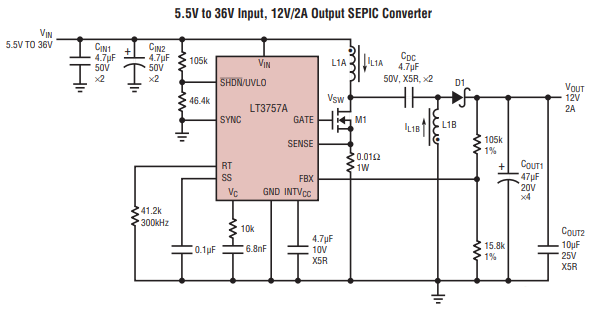
\includegraphics[height=7cm]{img/Referenzschaltung_SEPIC.PNG}
	\end{adjustbox}
	
		\subsection{Schaltung}
			\subsubsection{LTSpice}
			\begin{adjustbox}{center,caption={Simulationsschaltung des Analogteils in LTSpice},label={fig:LTSpice-Schaltung-Analogteil},nofloat=figure,vspace=\bigskipamount}
				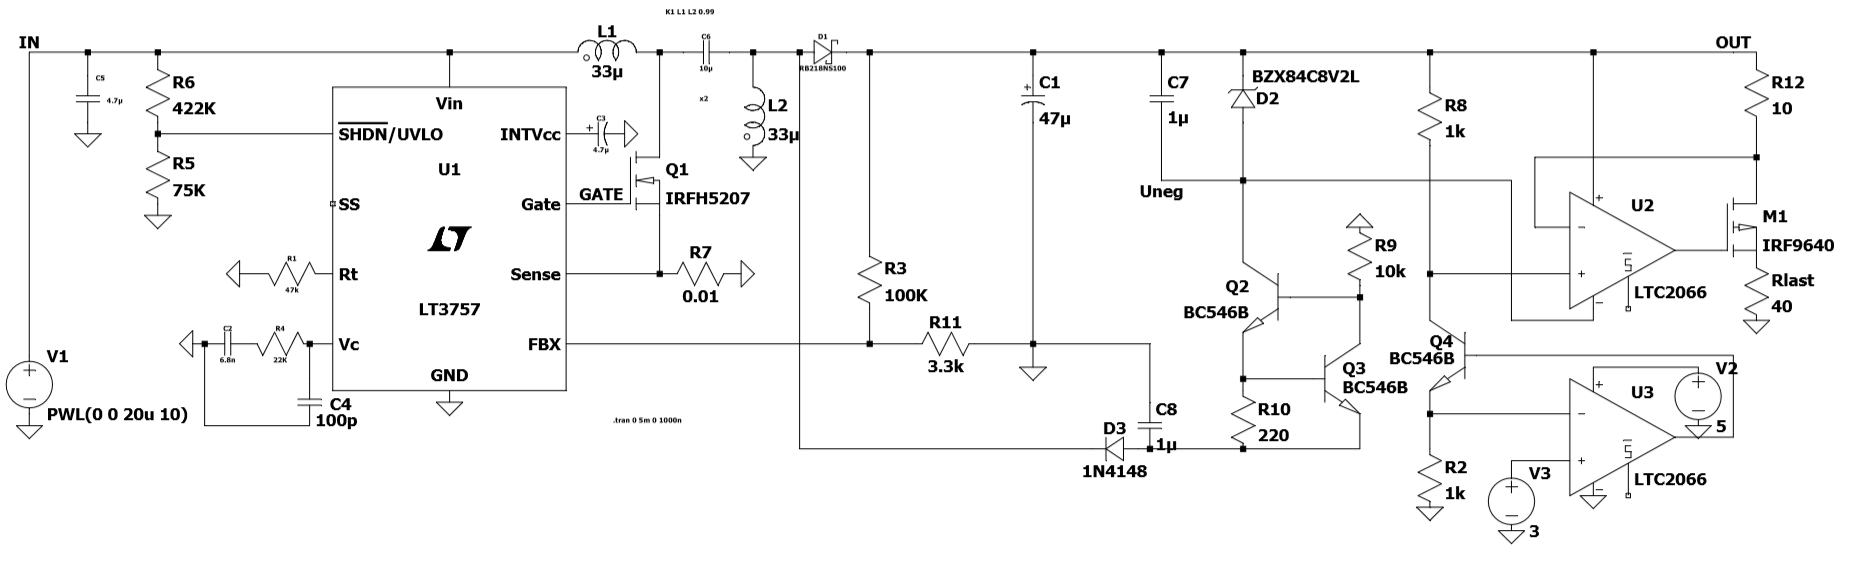
\includegraphics[width=\textwidth]{img/LTSpice_Schaltung_Analogteil.PNG}
			\end{adjustbox}
			\pagebreak
			\subsubsection{Altium}
			Die Schaltung in Altium wurde für eine bessere Übersicht in mehrere Teile aufgeteilt. Um trotzdem die Verbindung zwischen den einzelnen Leitungen herzustellen wurden sogenannte Ports verwendet, das sind Verbindungen mit Gleichnamigen Kästchen.
			\paragraph{SEPIC}
			\begin{adjustbox}{center,caption={Grundbeschaltung des LT3757},label={fig:LT3757-Grundbeschaltung},nofloat=figure,vspace=\bigskipamount}
				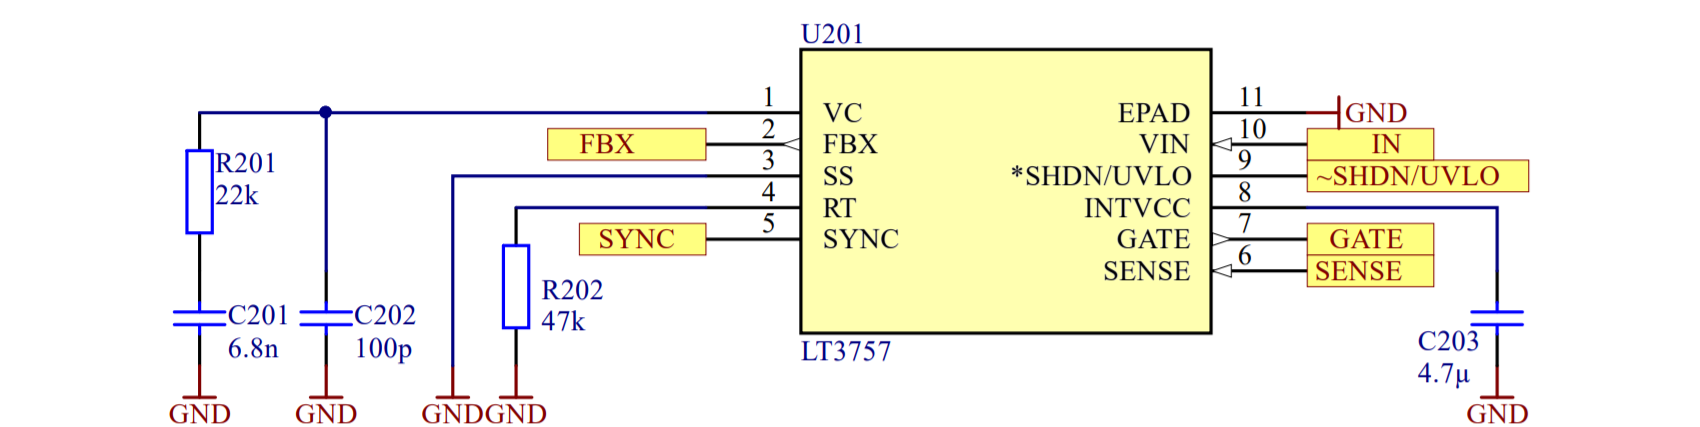
\includegraphics[width=\textwidth]{img/SEPIC_Altium.PNG}
			\end{adjustbox}
			Oben abgebildet ist die Grundbeschaltung des SEPIC-Chip LT3757. Das RC-Netzwerk bei dem VC-Pin hält die Spannung für die Erzeugung der Internen Spannung stabil erzeugt wird stabil gehalten werden kann. Am RT-Pin wird mittels des Wiederstandes eine Schaltfrequenz eingestellt. Der Pin INTVCC ist da um die Spannungen für die Interne Versorgung und das Gate stabil zu halten.
			\paragraph{Undervoltage Shutdown für SEPIC}
			\begin{adjustbox}{center,caption={Undervoltage Shutdown SChaltung für LT3757},label={fig:uvlo},nofloat=figure,vspace=\bigskipamount}
				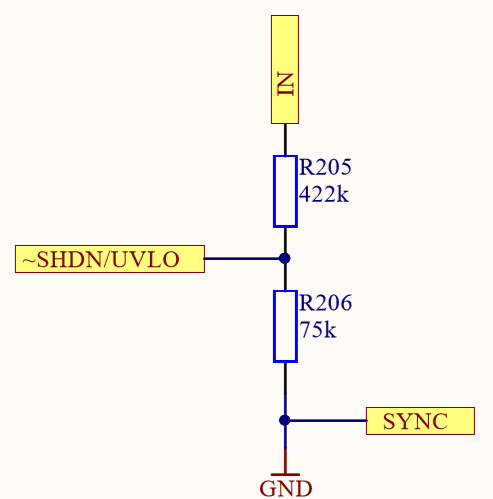
\includegraphics[height=6cm]{img/Undervolteage_Shutdown_SEPIC.PNG}
			\end{adjustbox}
			Dieser Teil der Schaltung ist dafür zuständig, dass die Spannung am Eingang überprüft wird, wenn die Spannung zu klein ist, wird der SEPIC-Chip deaktiviert um keine Schäden verursachen zu können.
			\pagebreak
			\paragraph{Feedback Schaltung für SEPIC}
			\begin{adjustbox}{center,caption={Feedback Schaltung für SEPIC},label={fig:feedback},nofloat=figure,vspace=\bigskipamount}
				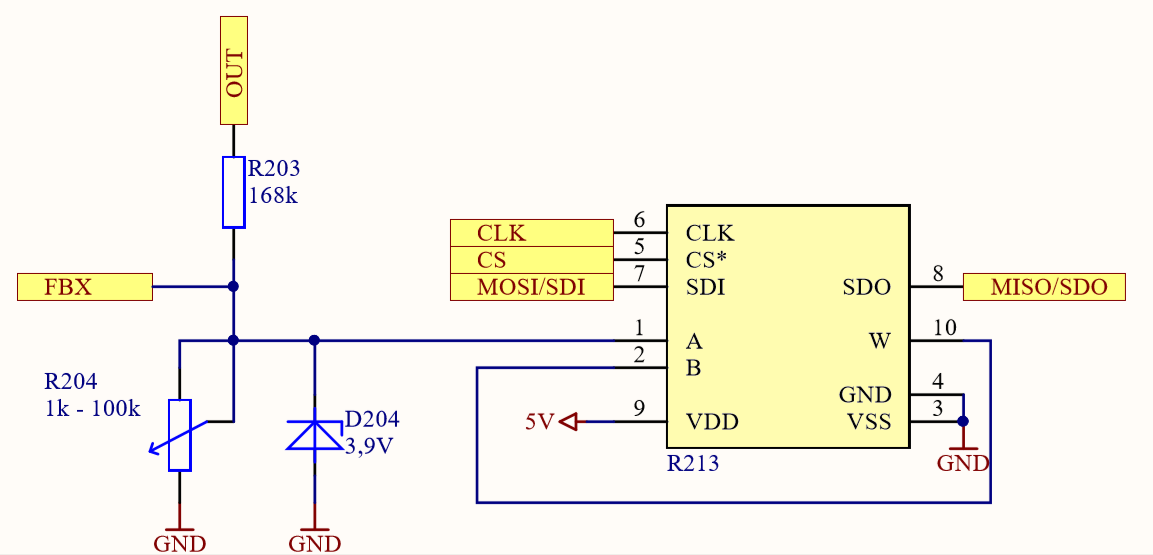
\includegraphics[height=6cm]{img/Feedback_SEPIC.PNG}
			\end{adjustbox}
			Dieser Teil ist zuständig für das Feedback der Spannung, die die Schaltfrequenz des FETs einstellt, über den auch die Ausgangsspannung eingestellt wird.
			\paragraph{Regelung für SEPIC}
			\begin{adjustbox}{center,caption={Regelungsschaltung für LT3757},label={fig:regelung},nofloat=figure,vspace=\bigskipamount}
				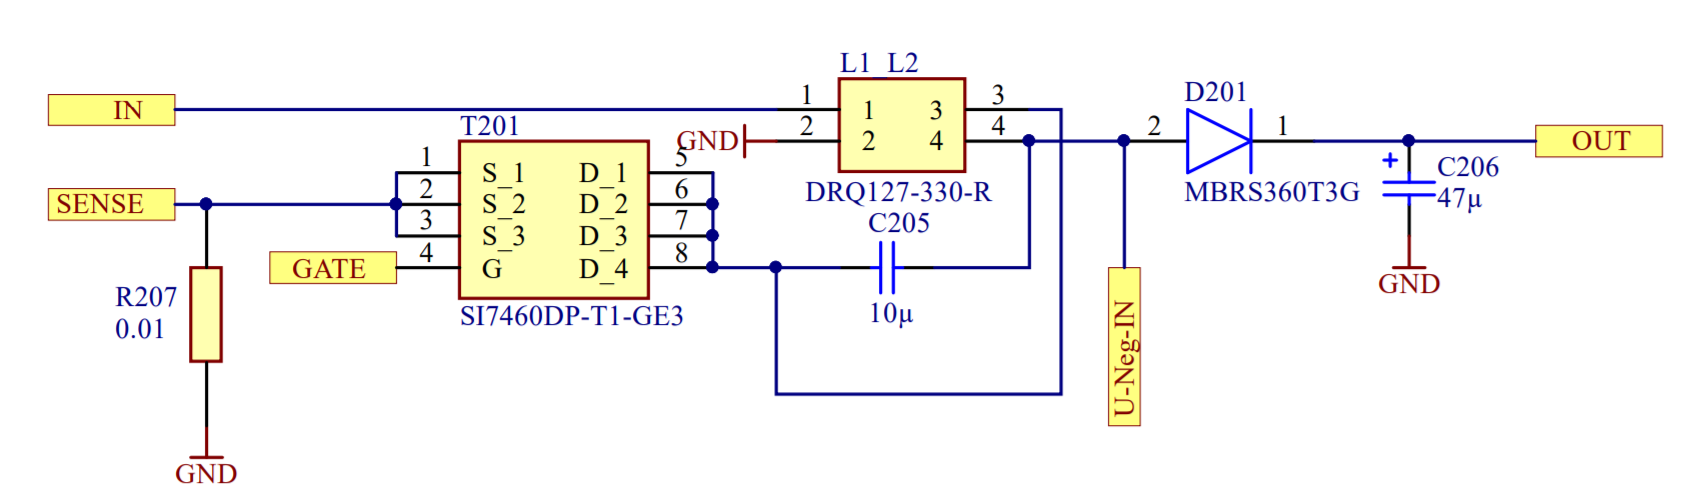
\includegraphics[width=\textwidth]{img/Regelung_SEPIC.PNG}
			\end{adjustbox}
			\pagebreak
			\paragraph{Negative Spannung}
			\begin{adjustbox}{center,caption={Schaltung für Versorgung von OPV der Stromquelle},label={fig:neg-spg},nofloat=figure,vspace=\bigskipamount}
				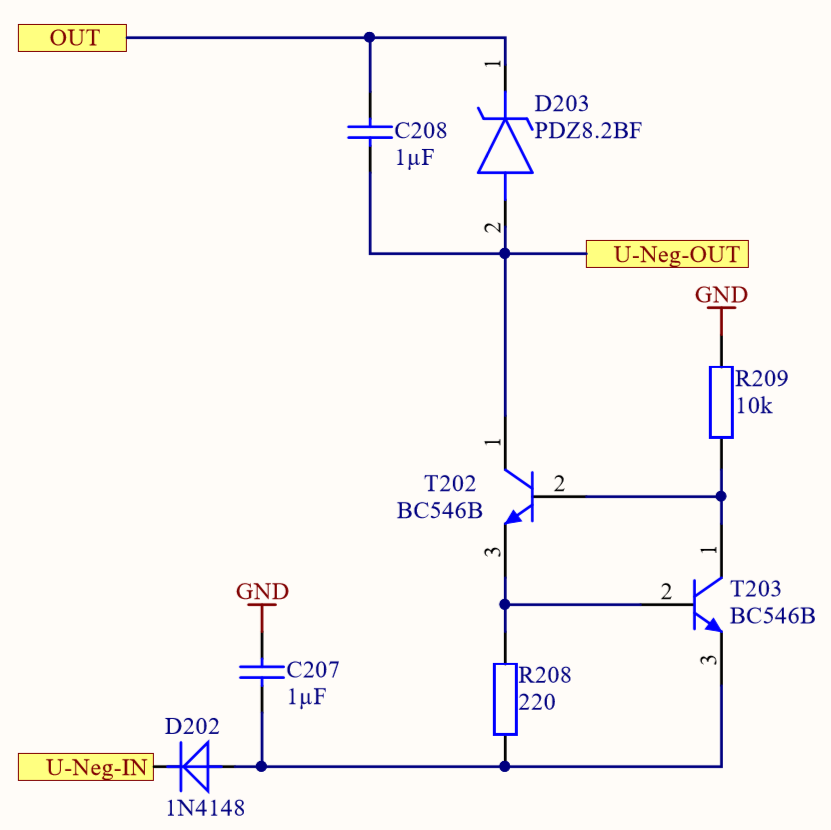
\includegraphics[height=10cm]{img/Negative_Spannung.PNG}
			\end{adjustbox}
			\paragraph{Stromquelle}
			\begin{adjustbox}{center,caption={Schaltung für die Einstellbare Stromquelle},label={fig:stromquelle},nofloat=figure,vspace=\bigskipamount}
				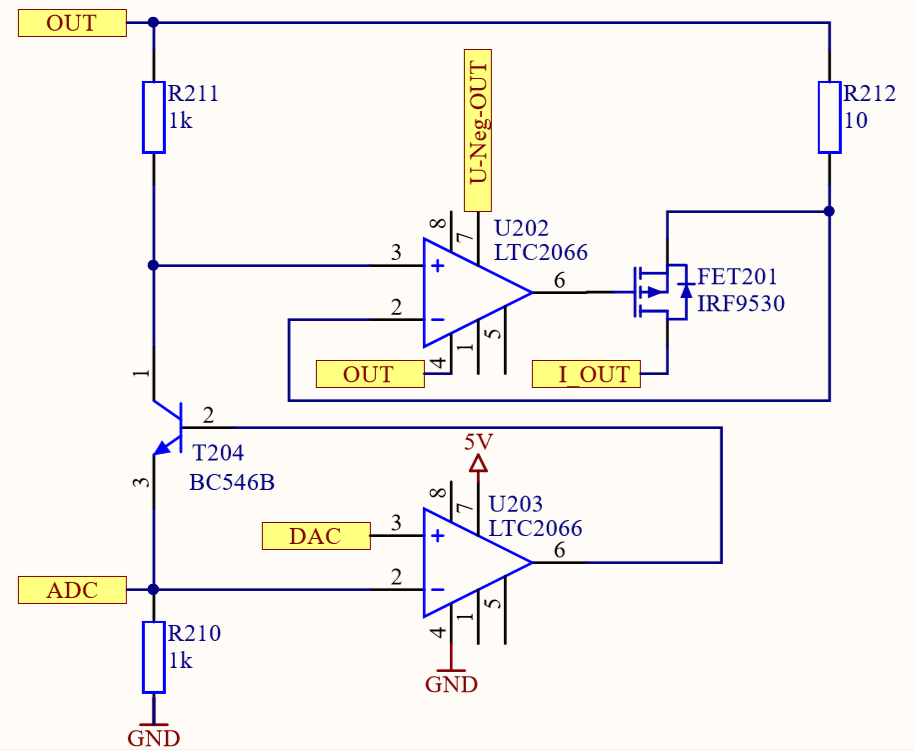
\includegraphics[height=8cm]{img/Stromquelle_SEPIC.PNG}
			\end{adjustbox}
			
			
		\subsection{Simulationen}
			\begin{adjustbox}{center,caption={Simulation der Schaltung Mittels LTSpice},label={fig:LTSpice-Simulation-1},nofloat=figure,vspace=\bigskipamount}
				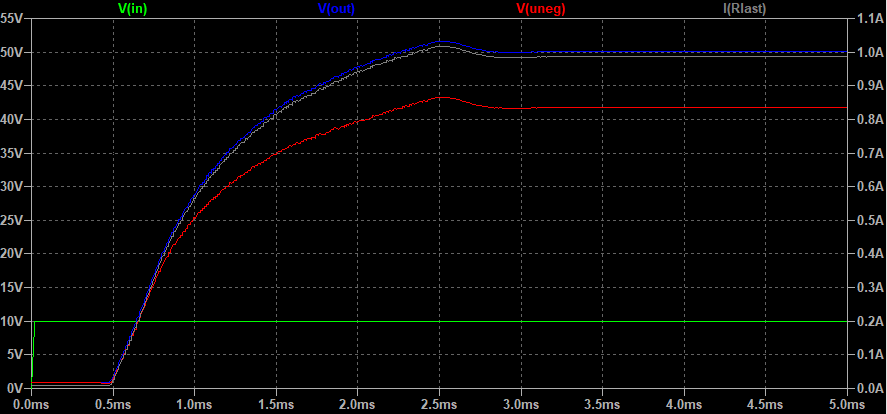
\includegraphics[width=\textwidth]{img/LTSpice_Simulation_1.PNG}
			\end{adjustbox}
			Wie in Abbildung \ref{fig:LTSpice-Simulation-1} zu sehen, ist in der Simulation die Eingangsspannung(in) auf 10 Volt eingestellt, der SEPIC-Converter braucht hier ca. 2,75ms um die Ausgangsspannung(out) auf konstante 50 Volt einzustellen. Bei der Simulierten Belastung von 40 Ohm(Rlast) wird ca 1 Ampere aus der Schaltung gezogen. Das entspricht auch den Leistungsanforderungen der Firma, welche die maximale benötigte Ausgangsleistung mit 40 Watt angegeben hat. 
			
			\begin{align*} 
			P_{out} = U_{out} \cdot I_{Rlast} = 50V \cdot 1A = 50W
			\end{align*} 
			
			Laut Simulation hat diese Schaltung eine Ausgangsleistung von 50W, was sogar mehr ist als angegeben. 
	
	\section{Digitalteil}
		\subsection{Schaltung}


%% ANHANG ==============================================%%
\appendix

%% abkürzungsverzeichnis ===============================%%
%% start of file abkuerzungen.tex

% Abkuerzungsverzeichnis
\addchap{
	\iflanguage{english}{Acronyms}{Abkürzungsverzeichnis}}
\begin{acronym}[ACRONYM]
\acro{adc}[ADC]{Analog Digital Converter}
\acro{can}[CAN]{Controller Area Network}
\acro{dac}[DAC]{Digital Analog Converter}
\acro{ldo}[LDO]{Low-Dropout regulator}
\acro{lmm}[LMM]{LED Matrix Manager}
\acro{pcb}[PCB]{Printed Circuit Board}
\acro{sepic}[SEPIC]{Single Ended Primary Inductance Converter}
\acro{opv}[OPV]{Operationsverstärker}
\acro{fet}[FET]{Field-Effect Transistor}
\acro{led}[LED]{Light Emitting Diode}
\acro{z-diode}[Z-Diode]{Zener Diode}
\acro{r}[R]{Resistor}
\acro{c}[C]{Capacitor}
\acro{gper}[GPER]{General Purpose Enable Register}
\acro{canif}[CANIF]{Control Area Network Interface}
\acro{cancfg}[CANCFG]{Control Area Network Configuration}
\acro{canctrl}[CANCTRL]{Control Area Network Controll}
\acro{mbits}[Mbit/s]{Megabit pro Sekunde}
\acro{mosi}[MOSI]{Master Out Slave In}
\acro{miso}[MISO]{Master In Slave Out}
\acro{sda}[SDA]{Serial Data Out}
\acro{sdi}[SDI]{Serial Data In}
\acro{ucd}[UCD]{User Controlled Device}
\acro{led}[LED]{Light Emitting Diode}
\acro{mosfet}[MOSFET]{Metal–Oxide–semiconductor Field-Fffect Transistor}
\acro{fet}[FET]{Field-Fffect Transistor}
\acro{gpio}[GPIO]{General Purpose In Out}
\acro{i/o}[I/O]{In/Out}
\acro{tdr}[TDR]{Transmit Data Register}
\end{acronym}\newpage

%% end of file abkuerzungen.tex
%%======================================================%%

%% abbildungsverzeichnis ===============================%%
\setcounter{lofdepth}{2}
\dipalistoffigures
%%======================================================%%

%% tabellenverzeichnis =================================%%
\setcounter{lotdepth}{2}
\dipalistoftables
%%======================================================%%

%% danksagungen=========================================%%
%%\begin{acknowledgements}
	\begin{center}
    Wir danken allen die die uns mit Ratschlägen und Ideen bei unserer Arbeit geholfen haben. Besonderer Dank fällt an Dipl.-Ing. Josef Radlbauer, der uns als Betreuer unserer Diplomarbeit immer wieder mit Ratschlägen und Ideen zur Seite Stand. Wir danken auch Dipl.-Ing. Markus Tillich für Tipps und Ratschläge beim Schaltungsdesign des Schaltwandlers. Besonderer Dank fällt auch an Ing. Rudolf Janeczek BEd MSc, der für uns den Kontakt mit der Firma ZKW aufgebaut hat, die uns mit der Idee für die Diplomarbeit betraut machten. Den Vertreten der Firma ZKW, Matthäus Artmann und Daniel Seitl, welche unsere Hauptansprechpartner waren, möchten wir besonders danken. 
	\end{center}
\end{acknowledgements}
%% Für Diplomarbeit hinzufügen
%%======================================================%%

%% literaturverzeichnis ================================%%
%%\newewpage
%%\begin{literature}
% The TeXbook by D. E. Knuth
\bibitem[1]{TeXbooooook}{\textbf{Donald~E.~Knuth:} \emph{The \TeX{}book}. 1986, {\scshape Addison--Wesley} Verlag,\\ ISBN-13: 978-0-201-13447-6}

\end{literature}
 
%%======================================================%%

%% betreuungsprotokolle ================================%%
%%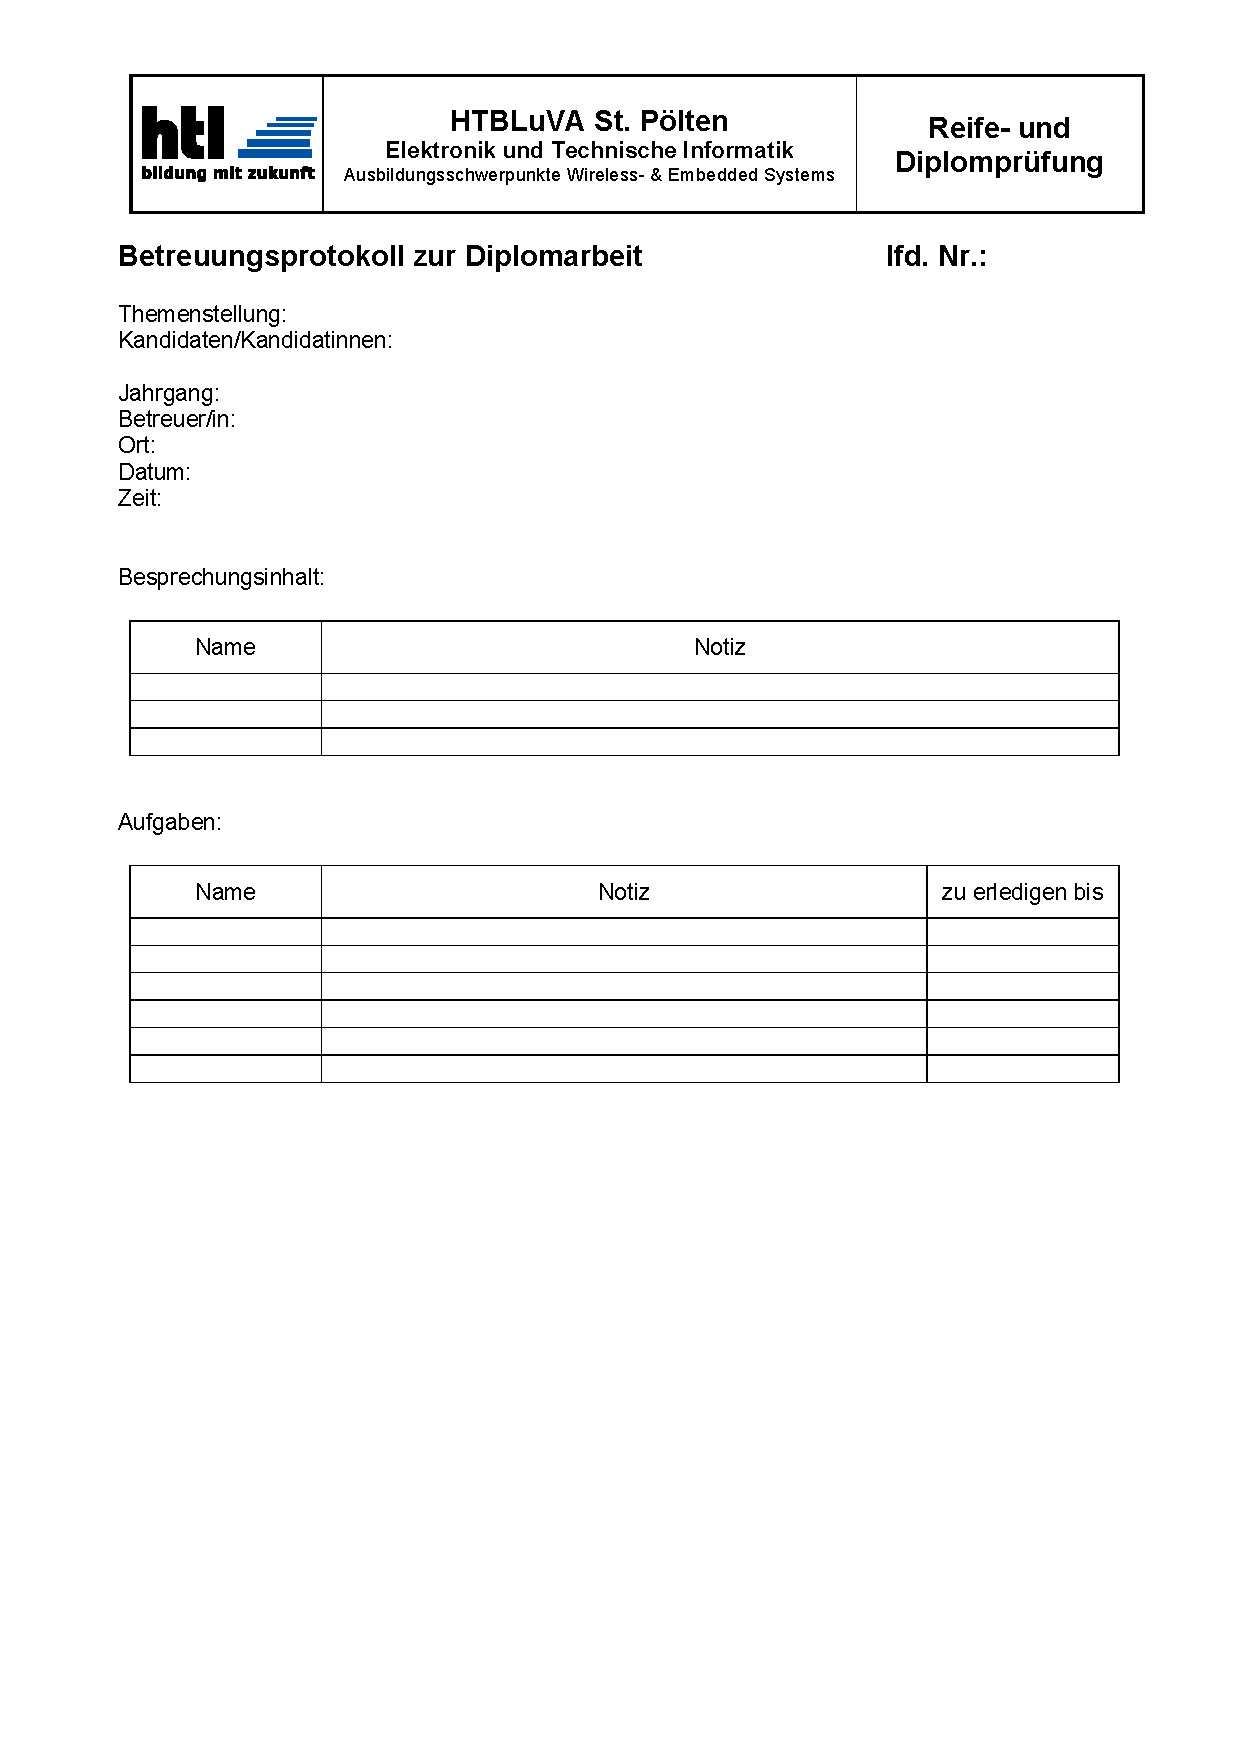
\includepdf[pages=-]{form/betreuungsprotokoll_1.pdf} Noch hinzufügen
%% =====================================================%%

\end{document}
